\section*{Généralités}
\label{sec:generalites}
\addcontentsline{toc}{section}{Généralités}

\subsection*{Les examens professionnels}
\label{subsec:examsprofs}
\addcontentsline{toc}{subsection}{Les examens professionnels}
\captionsetup{justification=centering}
Bien souvent, les examens professionnels sont l'une des premières choses dont l'on entend parler lorsqu'il est question d'actuariat. Il y a beaucoup d'informations disponibles sur le sujet, autant à partir de sources officielles que sur différents forums de discussion.\vspace{\baselineskip}

Afin d'avoir une bonne idée du cheminement, je vous suggère de vous référer en premier lieu aux informations se trouvant sur les sites des deux principales organisations professionnelles en actuariat: la \href{https://soa.org/member/}{\emph{Society of Actuaries (SOA)}} et la \href{http://www.casact.org/}{\emph{Casualty Actuarial Society (CAS)}}. Essentiellement, ce sont leurs champs d'activité différents qui distinguent ces deux organisations:
\begin{itemize}
\item La CAS se spécialise dans l'assurance IARD (Incendie, accident et risques divers).
\item La SOA regroupe les branches assurance-vie, retraite, assurance-maladie, investissement et gestion de risques en entreprise.\footnote{ Il est à noter que la spécialisation \emph{General Insurance} de la SOA n'est pas reconnue par l'Institut canadien des actuaires (ICA).}
\end{itemize}
\vspace{\baselineskip}

Vous remarquerez qu'il y a, autant du côté de la CAS que de la SOA, une série d'examens préliminaires suivie par des examens avancés. Certains examens préliminaires sont communs à tous, peu importe la spécialisation que l'on désire atteindre. Ces examens sont P/1, FM/2 et IFM/3F. La raison pour laquelle il y a deux appellations par examen préliminaire est que la SOA et la CAS ne nomment pas de la même façon ces examens dans leur cheminement. Du côté de la SOA, on a les examens P, FM et IFM, alors que ces mêmes examens se nomment 1, 2 et 3F du côté de la CAS. La section \nameref{sec:prelims} du présent document parlera plus en détails du contenu de ces examens, du matériel d'étude à utiliser et des façons de bien s'y préparer.\vspace{\baselineskip}

Après ces examens communs aux deux sociétés, il y a d'autres examens préliminaires à accomplir, mais ces examens sont différents selon que l'on suive le chemin de la SOA ou de la CAS. Du côté de la SOA, il faut réussir les examens STAM, LTAM, SRM et PA. Quant à la CAS, elle exige la réussite des examens MAS-I, MAS-II, 5 et 6. Une fois ces examens préliminaires réussis et d'autres exigences satisfaites\footnote{Ces exigences supplémentaires sont des crédits VEE (voir la section \nameref{subsec:vee}), des modules d'apprentissage en ligne et des séminaires de professionnalisme. Les exigences supplémentaires de la SOA et de la CAS diffèrent sur plusieurs points.}, le candidat atteint le rang d'Associé (ASA ou ACAS selon la société choisie), qui est le but à moyen terme de la plupart des étudiants et des récents gradués en actuariat. \vspace{\baselineskip}

Une fois le titre d'Associé atteint, d'autres examens attendent ceux qui veulent aller plus loin. Ce sont les examens avancés, qui une fois réussis, permettent au candidat d'atteindre le titre de Fellow (FSA ou FCAS, encore une fois selon la société choisie). Vous aurez peut-être remarqué que même si la SOA regroupe plusieurs branches assez distinctes, elle offre les mêmes examens préliminaires à tous ses candidats. Ce sont donc plutôt les examens avancés qui permettent d'atteindre une spécialisation dans cette société. Pour ce qui est de la CAS, comme c'est une société qui est déjà spécialisée dans une seule branche, les examens avancés sont communs à tous. Le présent document ne traitera pas de chacun des examens avancés en détail, en raison du nombre très élevé d'examens différents et du fait que le document s'adresse surtout à des apprentis actuaires qui ont réussi peu ou pas d'examens. Toutefois, vous pouvez consulter la \nameref{subsec:faq} si les détails techniques de ces examens avancés vous intéressent. \vspace{\baselineskip}

Vous pouvez visualiser la progression nécessaire (examens préliminaires, autres exigences et examens avancés) jusqu'au titre de Fellow, autant pour la SOA que pour la CAS, dans la figure de la page suivante. \newpage

\begin{center}
\begin{figure}[hp]
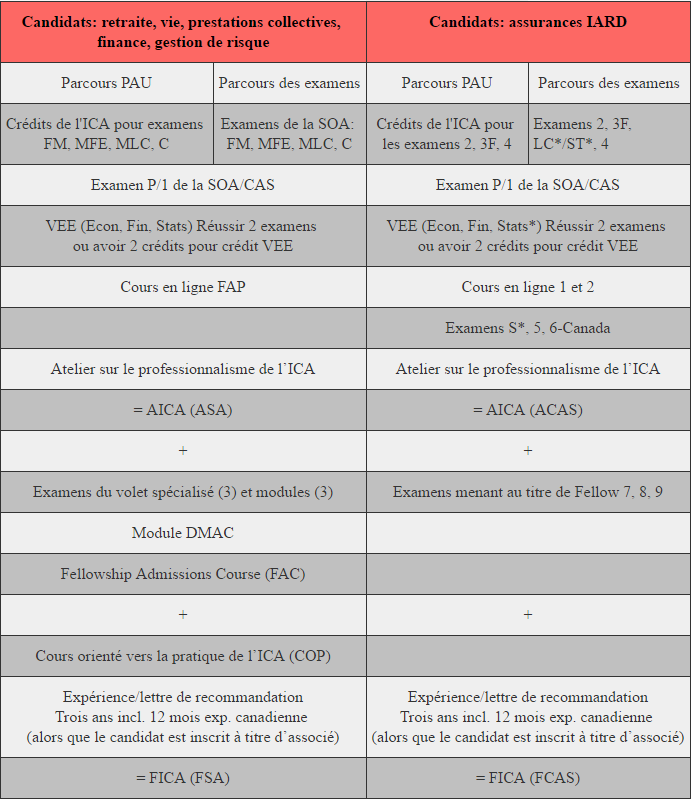
\includegraphics[width=1\textwidth]{tableau_ICA.png}
\caption{Cheminement professionnel en actuariat --- Grille fournie par Joseph Gabriel de l'Institut canadien des actuaires}
\end{figure}
\par
\end{center}


Autre élément important à savoir: le 1er juillet 2018, les exigences à satisfaire pour devenir Associé de la SOA ont subi des changements importants. Le syllabus de la plupart des examens ont été modifiés, les exigences des VEE ont changé et deux examens complètement nouveaux ont été créés. Ces changements sont mentionnés pour chaque examen et VEE en question lorsqu'il est traité. Pour avoir plus d'informations sur les changements de juillet 2018 et pour connaître la réponse de la CAS à ces changements, vous pouvez consulter la sous-section \nameref{subsec:changeasa} du présent document. \vspace{\baselineskip}

Il y a énormément d'informations sur les sites de la SOA et de la CAS, mais ils ne disent pas tout non plus. La SOA parle souvent  d'une \emph{règle du pouce} d'environ 100 heures d'étude par heure d'examen, sans donner de détails vraiment sur la façon de répartir ces heures ou quel matériel d'étude utiliser par exemple. Les différents forums de discussion sont une excellente ressource pour connaître ce genre d'informations, les deux principaux étant \href{http://www.actuarialoutpost.com/}{\emph{Actuarial Outpost}} et \href{https://www.reddit.com/r/actuary}{\emph{/r/actuary}}. La page \href{https://www.reddit.com/r/actuary/wiki/index#wiki_the_frequently_asked_questions_.28faqs.29}{\emph{FAQ}} de \emph{/r/actuary} contient beaucoup d'informations utiles pour les gens qui débutent en actuariat. Également, la discussion \href{https://www.reddit.com/r/actuary/comments/1enzdd/how_long_to_get_to_asa_is_two_years_possible/}{\emph{How long to get to ASA}} de ce même site contient des réponses intéressantes au sujet du temps nécessaire pour compléter les examens. \vspace{\baselineskip}

Pour connaître des statistiques au sujet des examens professionnels, vous pouvez consulter le site \href{http://actuarial-lookup.com/}{\emph{actuarial-lookup}}. Ce site contient des données de 2007 jusqu'à aujourd'hui. \vspace{\baselineskip}

Vous trouverez les dates importantes pour les examens préliminaires sur cette \href{https://www.soa.org/Education/Exam-Req/Exam-Day-Info/edu-2018-cbt-test-schedule.aspx}{page}. J'en profite également pour mentionner qu'en vous inscrivant avec votre adresse courriel universitaire, vous serez éligible à un rabais étudiant pour les examens IFM/3F, STAM/4 et LTAM. Voir cette \href{https://soa.org/Education/Exam-Req/Syllabus-Study-Materials/Exam-and-Module-Fees.aspx}{page} pour plus de détails concernant les coûts d'inscription. \vspace{\baselineskip}

\newpage

\subsection*{L'ICA et les accréditations d'examens professionnels}
\label{subsec:ica}
\addcontentsline{toc}{subsection}{L'ICA et les accréditations d'examens professionnels}

Une autre organisation est d'une grande importance pour les étudiants canadiens en actuariat: il s'agit de \href{https://www.cia-ica.ca/fr/accueil}{l'Institut canadien des actuaires (ICA)}. Là où la SOA et la CAS gèrent plutôt l'aspect académique de la profession, l'ICA s'occupe surtout de l'aspect professionnel et du droit de pratique des actuaires canadiens. Il y a également des titres d'Associé et de Fellow de l'ICA (AICA et FICA), mais il ne faut pas réussir d'autres examens pour avoir ces titres; en effet, ils sont \textit{associés} aux titres d'Associé et de Fellow obtenus dans une autre société (SOA ou CAS). En d'autres mots, les étudiants en actuariat font des examens pour obtenir des titres de la SOA ou de la CAS, et une fois ces titres obtenus, les titres correspondants de l'ICA viennent automatiquement avec. \vspace{\baselineskip} 

Le tableau ci-dessous a pour but de clarifier les différences entre les rôles des trois organismes mentionnés jusqu'à présent.

\begin{center}
\begin{figure}[hp]
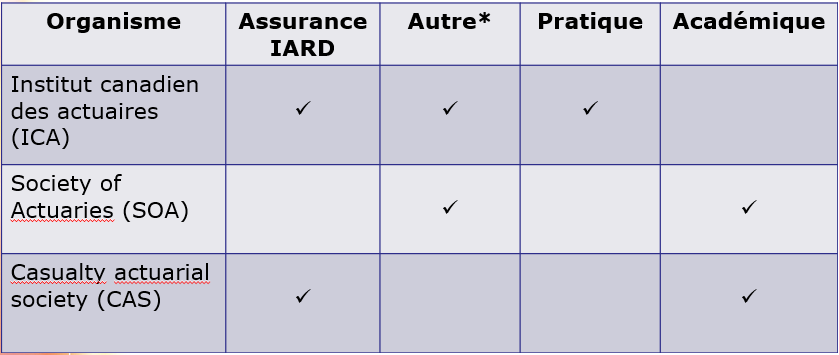
\includegraphics[width=1\textwidth]{roles_organismes.png}
\caption{Différences entre les rôles de la SOA, de la CAS et de l'ICA}
\end{figure}
\par
\end{center}

Il y a quelques années, l'ICA a lancé un programme d'accréditation des examens professionnels. Ce projet vise à valoriser davantage les connaissances apprises lors de l'éducation supérieure et à permettre aux étudiants de ne pas avoir à être testés deux fois sur les mêmes connaissances (une fois à l'école et une autre fois dans les examens professionnels). De fait, si un étudiant a des notes jugées adéquates à certains cours qui sont associés à un certain examen professionnel, alors l'étudiant peut se faire \textit{accréditer} l'examen professionnel et ne pas avoir du tout à le faire. Par contre, si les notes requises ne sont pas atteintes dans les cours en question, l'étudiant ne peut pas se faire accréditer l'examen professionnel et il doit le tenter et le réussir. \vspace{\baselineskip}

Vous trouverez l'information quant aux cours qui permettent d'obtenir les accréditations d'examen de l'ICA dans votre \href{https://www.act.ulaval.ca/programmes-et-cours/premier-cycle/guide-de-letudiant/}{guide de l'étudiant}. Cette information se trouve généralement dans les dernières pages du document. Remarquez que tous les examens préliminaires de la SOA sont accréditables, sauf le premier examen (\nameref{subsec:examp}). \vspace{\baselineskip}

Il est important de savoir que la CAS reconnaît les accréditations de l'ICA, mais que la SOA ne les reconnaît pas encore. Ainsi, un candidat qui obtient des accréditations pour certains examens peut obtenir les titres de Fellow de l'ICA et de la CAS mais, s'il est du côté de la SOA, il ne pourra pas devenir Fellow de la SOA --- il sera seulement Fellow de l'ICA. En théorie, cela ne devrait pas être grave puisque c'est l'ICA qui gère le droit de pratique au Canada et pas la SOA. Cependant, ce ne sont pas toutes les entreprises qui voient d'un bon œil le fait de s'être fait accréditer des examens professionnels et de ne pas avoir les titres de la SOA. La décision de prendre les accréditations d'examens ou non reste à la discrétion de chaque étudiant et je vous conseille de bien vous informer à ce sujet et de peser le pour et le contre selon votre avancement et vos intérêts.

\newpage

\subsection*{Les crédits VEE}
\label{subsec:vee}
\addcontentsline{toc}{subsection}{Les crédits VEE}
Les crédits VEE (\emph{Validation by Educational Experience}) sont une composante nécessaire pour obtenir le titre d'Associé. Les VEE permettent de couvrir des sujets qui ne sont pas formellement testés lors des examens préliminaires. La CAS et la SOA ont deux VEE en commun: le VEE \emph{Corporate Finance and Accounting} et le VEE \emph{Economics}. La SOA compte également le VEE \emph{Applied Statistical Methods}. Anciennement, la CAS comptait également ce troisième VEE, mais ils ont décidé de l'enlever suite à la création de l'Examen S (maintenant MAS-1).\vspace{\baselineskip}

Les crédits VEE peuvent être complétés en obtenant une note d'au moins B- dans certains cours du baccalauréat. Présentement, les cours qui permettent d'obtenir les VEE sont:
\begin{itemize}
\item Pour le VEE \emph{Applied Statistical Methods}, \textit{ACT-2000 Analyse statistique des risques actuariels}. Avant le 1er juillet 2018, c'étaient les cours \textit{ACT-2003 Modèles linéaires en actuariat} \textbf{et} \textit{ACT-2010 Séries chronologiques} qui procuraient le VEE.
\item Pour le VEE \emph{Economics}, \textit{ECN-1000 Principes de microéconomie} \textbf{et} \textit{ECN-1010 Principes de macroéconomie}. 
\item Pour le VEE \emph{Corporate Finance and Accounting}, \textit{ACT-1006 Gestion du risque financier I} \textbf{et} \textit{CTB-1000 Comptabilité générale}. La partie \emph{Accounting} du VEE sera nécessaire à partir du 1er juillet 2019. Également, la partie \emph{Corporate Finance} sera allégée à partir du 1er juillet 2019 (il faudra des cours de finance moins avancés pour obtenir le VEE à partir de cette date), car les éléments de finance plus avancés auront plutôt été distribués dans les différents examens professionnels. Remarquez que les changements de ce VEE seront effectifs à partir du 1er juillet 2019, et pas à partir du 1er juillet 2018 comme pour les autres VEE et examens.
\end{itemize}
\vspace{\baselineskip}

Comme vous pouvez le constater, les VEE ont subi plusieurs modifications suite aux changements des prérequis pour devenir Associé de juillet 2018. Pour ceux qui auraient des questions sur les transitions des cours qui procurent les VEE, n'hésitez pas à nous contacter. \vspace{\baselineskip}

Advenant le cas où vous n'auriez pas la cote minimale pour obtenir le crédit, vous devrez éventuellement compléter un cours en ligne sur le sujet du VEE en question, lequel sera suivi d'un examen.

\newpage

\subsection*{Alternatives et compléments aux manuels}
\label{subsec:alternatives}
\addcontentsline{toc}{subsection}{Alternatives et compléments aux manuels}
Il existe quelques alternatives et compléments aux manuels d'étude. Par exemple, les sites \href{http://www.theinfiniteactuary.com/}{\emph{The Infinite Actuary}} et \href{https://www.coachingactuaries.com/}{\emph{Coaching Actuaries}} offrent des formations préparatoires sous forme de vidéos pour tous les examens préliminaires (et certains examens avancés dans le cas de \emph{The Infinite Actuary}). Ces ressources sont toutefois peu populaires auprès des étudiants du baccalauréat, puisqu'elles sont souvent dispendieuses.\vspace{\baselineskip}

Un complément incontournable aux manuels d'étude est le système dynamique de génération d'examens ADAPT. Ce système est offert par le site \href{https://www.coachingactuaries.com/}{\emph{Coaching Actuaries}} et comporte une énorme banque de questions pour chacun des examens préliminaires. Le fonctionnement de ADAPT est plutôt simple; on débute au niveau 3, le système génère des examens pour vous et, dépendamment de votre résultat à l'examen, votre niveau (\emph{Earned Level} en anglais) va augmenter ou diminuer. Le niveau de l'examen correspond à sa difficulté; plus il est élevé, plus il sera difficile. Vous pourrez également plus facilement voir quelles sont les sections de l'examen où vous avez le plus de difficulté et créer des quiz spécifiquement sur ces sections afin de vous améliorer. L'objectif est d'atteindre un niveau 7 (sans tricher --- évidemment), puisque les statistiques disponibles montrent qu'environ 90\% des gens qui ont atteint ce niveau ont réussi leur examen. Vous aurez aussi droit à un rabais de 20\% pour les examens P, FM, IFM (MFE) grâce au code LAVALPC20 et un rabais de 30\% pour les examens C (STAM/MAS-2), MLC (LTAM), S (MAS-1) grâce au code LAVALPC30. Voir ce \href{https://www.youtube.com/watch?v=ZBxLa2J5jhs}{vidéo} pour une brève présentation de ADAPT. \vspace{\baselineskip}

L'association étudiante offre les manuels d'études P/1, FM/2, MFE/3 et S en version papier, ainsi que les livres pour les modules de la \textit{SOA} (\textit{FAP}). De plus, les manuels P/1, FM/2, MFE/3, C/4, S et MLC sont disponibles en version électronique sur le \href{https://drive.google.com/open?id=0B6kXivc6X9LISE1ydE41UnY3UDQ}{\textit{Google Drive}}. Également, prochainement les nouveaux livres d'étude seront disponibles pour les nouveaux examens et les nouvelles versions des examens.
\newpage